%\chapter{spacereq}

\label{ch:spacereq}

ProtoDUNE-SP is to be housed in an extension to the EHN1 hall in the North Area of the Pr\'{e}vessin site at CERN. 
The cryostat is constructed in a pit inside the building, surrounded on three sides by the pit walls.  On the fourth side of the cryostat, an ISO 8 clean room provides a space to construct, test and assemble the TPC and other components. 
A material pass-through structure called a \textit{sas}~\footnote{\textit{Sas} is a French word for a space outfitted with two doors, where one can only be opened if the other is closed; a sas used to pass between two spaces that must remain isolated from each other.} is adjacent to the clean room. Figure~\ref{fig:cryostat-in-ehn1} shows the layout of these structures in EHN1. A naming convention has been established for the four sides of the cryostat, shown in Figure~\ref{fig:cryo-side-names}.  The upper side is \textit{Jura}, the lower is \textit{Sal\`{e}ve}, the left is \textit{Beam}, and right is \textit{Downstream}.

%move this to installation 2/176/17 Anne: As detector materials are brought into EHN1, they are passed into the sas through its removable roof, then transported through a set of large doors from the sas into the clean room, where they are tested and assembled. When ready, each assembled TPC component passes through a temporary construction opening (TCO) in the cryostat for installation.
%While material is lowered into the sas from the gallery floor, the doors to the clean room remain closed to reduce contamination of the filtered air in the clean room.
%Once the roof of the sas is closed, these doors can be opened to move the material into the clean room.  

% moved down 2/16/17 The lighting inside the clean room and any temporary lighting inside the cryostat is filtered to limit the exposure of the PDS components to UV light.  Wavelengths below 450~nm are filtered out.   

\begin{cdrfigure}[ProtoDUNE-SP cryostat in EHN1]{cryostat-in-ehn1}{Layout of ProtoDUNE-SP cryostat, clean room and material sas in EHN1}
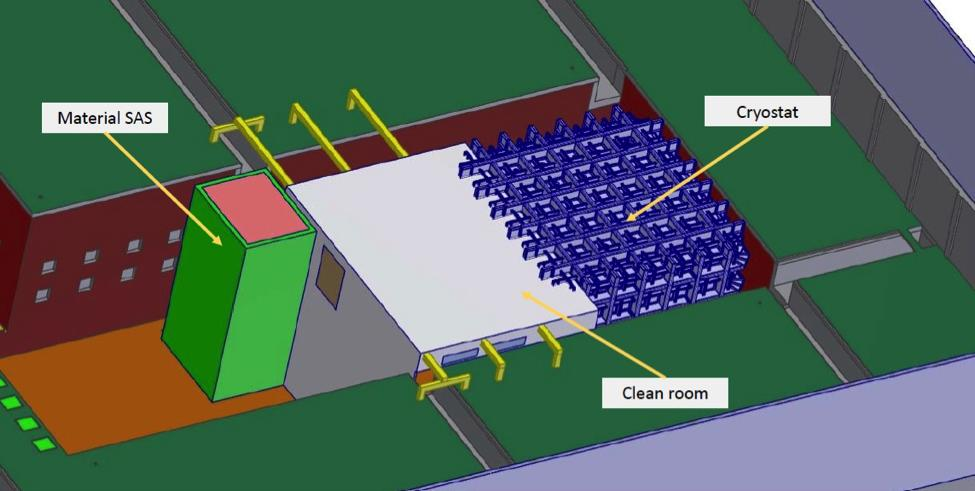
\includegraphics[width=0.8\textwidth]{sp-cryostat-in-ehn1}
\end{cdrfigure}


\begin{cdrfigure}[Conventions for labeling the four sides of the cryostat]{cryo-side-names}{Conventions for labeling the four sides of the cryostat}
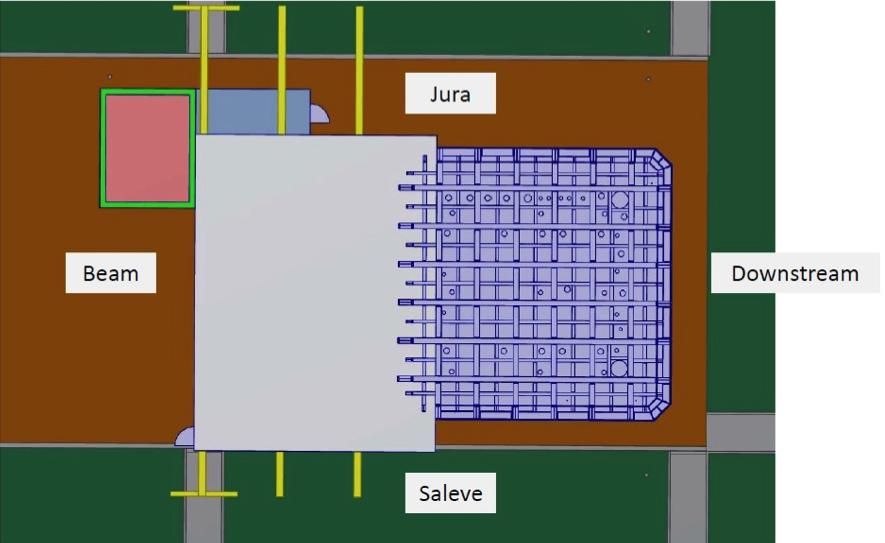
\includegraphics[width=0.8\textwidth]{naming-conv-cryo-sides}
\end{cdrfigure}

Figure~\ref{fig:elev-view-cryostat} shows an elevation section view of the cryostat indicating the position of the TCO and the location of the integrated cold testing stand (described in Section~\ref{sec:quality:space}).  

\begin{cdrfigure}[Elevation section view of the cryostat]{elev-view-cryostat}{Elevation section view of the cryostat}
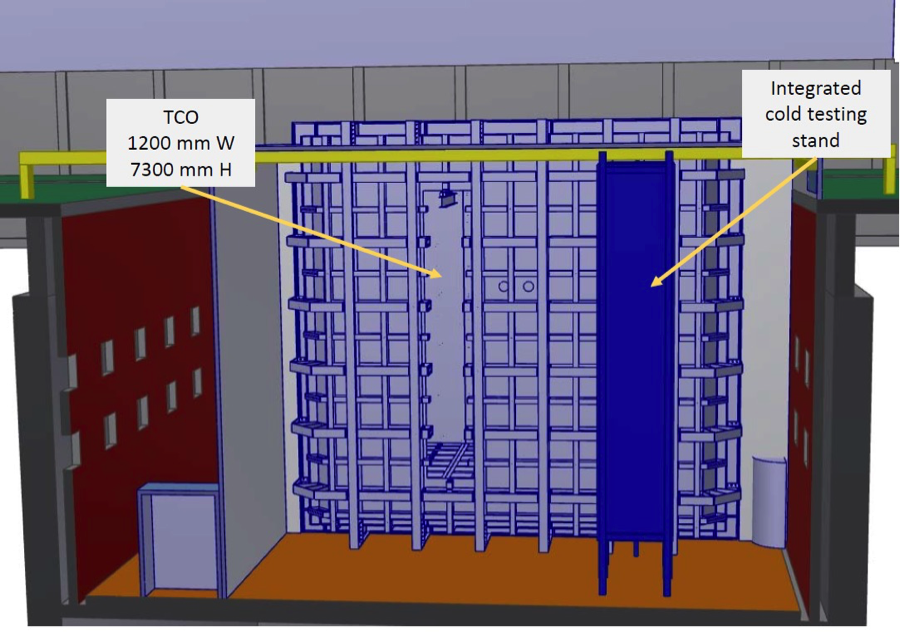
\includegraphics[width=0.8\textwidth]{elev-view-cryostat}
\end{cdrfigure}

Inside the clean room, a series of rails facilitate the movement of the detector components during the test and installation processes.  The conceptual layout of these rails is shown in Figure~\ref{fig:rails-in-cleanroom}.  The rails are positioned vertically at the same height as the detector support structure (DSS) rails inside the cryostat.  A temporary rail is installed through the TCO to bridge the DSS rails and clean room rails.  All the large components of the cryogenics piping and TPC are supported from these rails on movable trolleys as they are transported to the interior of the cryostat.  
Figure~\ref{fig:rails-in-cleanroom} also shows the approximate dimensions for the sas and the footprint of the clean room space.  These spaces are limited by the pit walls on two sides, and by the supports for the beam and beam instrumentation on the other. 


\begin{cdrfigure}[Layout of rails in clean room and dimensions]{rails-in-cleanroom}{Conceptual layout of rails in clean room to facilitate movement of TPC components; approximate dimensions for the material sas and the footprint of the clean room space are shown. (The supports for the beam and the beam instrumentation are not shown.)}
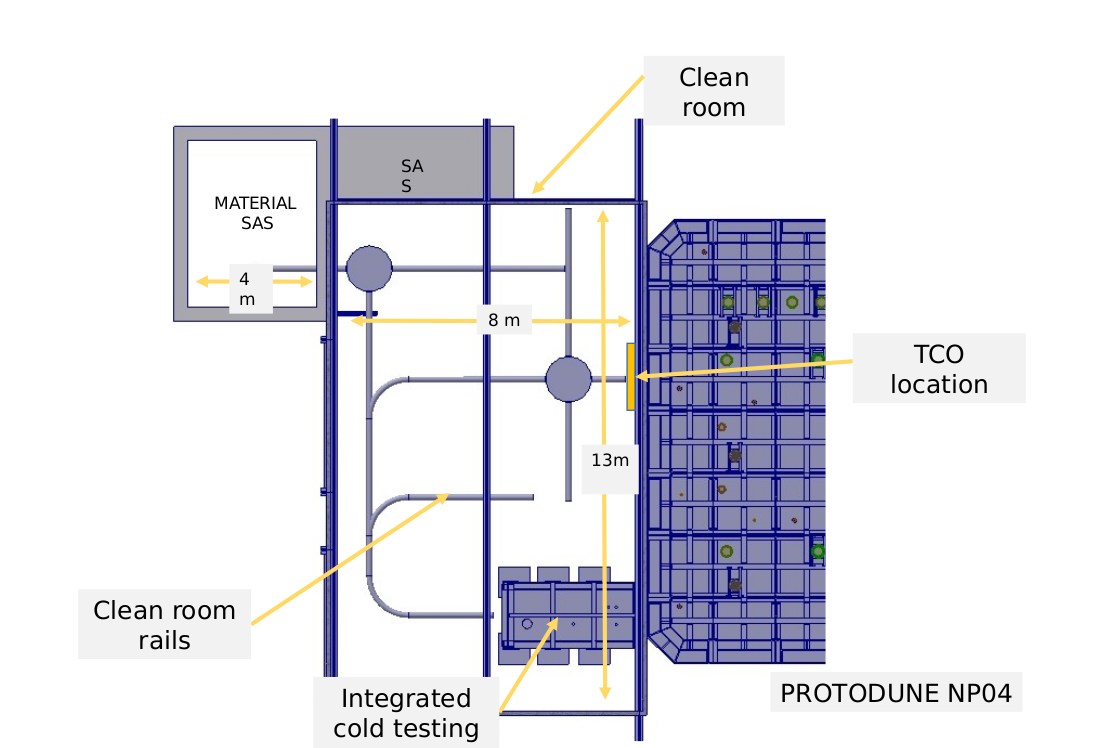
\includegraphics[width=0.9\textwidth]{CleanRoomLayout}
%\includegraphics[width=0.9\textwidth]{rails-in-cleanroom <--- old figure name}
\end{cdrfigure}

The lighting inside the clean room and any temporary lighting inside the cryostat is filtered to limit the exposure of the PDS components to UV light; wavelengths below 450~nm are filtered out. 


%\fixme{Anne moved the `planned locations for activities' to the installation chapter 2/16/17}
